\documentclass[9pt]{beamer}

% beamerthemeFeng.sty
% style file for beamer presentation

% tikz is used to ``draw'' title page and other templates in beamer
\usepackage{tikz,etoolbox}
\usetikzlibrary{shapes,arrows}

\definecolor{UWBlack}{HTML}{000000}
\definecolor{UWWhite}{HTML}{FFFFFF}


\definecolor{UWMathPinkL1}{HTML}{FFBEEF}
\definecolor{UWMathPinkL2}{HTML}{FF63AA}
\definecolor{UWMathPinkL3}{HTML}{DF2498}
\definecolor{UWMathPinkL4}{HTML}{C60078}
\definecolor{UWGrayL1}{HTML}{DFDFDF}
\definecolor{UWGrayL2}{HTML}{A2A2A2}
\definecolor{UWGrayL3}{HTML}{787878}
\definecolor{UWGrayL4}{HTML}{000000}
\definecolor{UWGoldL1}{HTML}{FFFFAA}
\definecolor{UWGoldL2}{HTML}{FFEA3D}
\definecolor{UWGoldL3}{HTML}{FFD54F}
\definecolor{UWGoldL4}{HTML}{E4B429}

\definecolor{carrot}{HTML}{EE693F}
\definecolor{ivory}{HTML}{F1F3CE}
\definecolor{emerald}{HTML}{265C00}
\definecolor{turquise}{HTML}{5BC8AC}
\definecolor{peacockblue}{HTML}{1E656D}
\definecolor{spicy}{HTML}{B51D0A}
\definecolor{bluegreen}{HTML}{5F968E}
\definecolor{rust}{HTML}{9B4F0F}
\definecolor{burntorange}{HTML}{DE7A22}
\definecolor{sea}{HTML}{20948B}
\definecolor{lagoon}{HTML}{6AB187}


% Set colors for different components in a slide
\setbeamercolor{background canvas}{bg=UWWhite}
\setbeamercolor{author}{fg=UWGoldL3}
\setbeamercolor{institute}{fg=UWMathPinkL3}
\setbeamercolor{title}{fg=UWGrayL4}
\setbeamercolor{section in head/foot}{bg=UWBlack, fg=UWGoldL3}
\setbeamercolor{author in head/foot}{fg=UWGoldL3, bg=UWBlack}
\setbeamercolor{title in head/foot}{fg=UWBlack,bg=UWGoldL3}
\setbeamercolor{institute in head/foot}{fg=UWGoldL3, bg=UWBlack}
\setbeamercolor{navigation symbols}{fg=UWBlack}
\setbeamercolor{normal text}{fg=UWGrayL3}
\setbeamercolor{section in toc}{fg=emerald}
\setbeamercolor{subsection in toc}{fg=bluegreen}
\setbeamercolor{frametitle}{fg=UWMathPinkL2, bg=UWGrayL1}
\setbeamercolor{block title}{bg=emerald, fg=ivory}
\setbeamercolor{block body}{bg=peacockblue!20, fg=peacockblue}
\setbeamercolor{section number projected}{bg=turquise,fg=black}
\setbeamercolor{block title example}{fg=rust,
	bg= sea!40}
\setbeamercolor{block body example}{fg= burntorange,
	bg= lagoon!20}

\setbeamerfont{frametitle}{series=\bfseries} % bold frame title
\setbeamerfont{section number projected}{% bold TOC bullet
  family=\rmfamily,series=\bfseries,size=\normalsize}
  
% two common fields in conference presentations
\newcommand\jointwork[1]{\def\insertjointwork{#1}}
\newcommand\conference[1]{\def\insertconference{#1}}

% Title page style
\setbeamertemplate{title page}{
\begin{tikzpicture}[remember picture, overlay]
\fill[UWWhite]
  ([yshift=30pt]current page.west) rectangle (current page.south east);

\fill[UWBlack]
  ([yshift=30pt]current page.west) rectangle (current page.north east);

\node[anchor=east] at ([yshift=-50pt,xshift=-15pt]current page.north east)
  {
  
\includegraphics[width=0.3\linewidth]{./hselogo_fullsize_inverted.png}};

\node[anchor=north west] at ([yshift=-70pt,xshift=15pt]current page.north west) (institute)
	{
	\parbox[t]{.78\paperwidth}{
    \usebeamerfont{institute}\usebeamercolor[fg]{institute}\large\bfseries\insertinstitute}
    };
    
\node[anchor=west] at ([yshift=-45pt,xshift=15pt]current page.north west) (author)
	{
	\parbox[t]{.78\paperwidth}{
    \usebeamerfont{author}\usebeamercolor[fg]{author}\Large\bfseries \insertauthor}
    };


    
\node[anchor=north] at ([yshift=15pt]current page.center) (title)
	{
	\parbox[t]{\textwidth}{\huge\bfseries\centering
	\usebeamerfont{title}\usebeamercolor[fg]{title}\inserttitle}
	};
    
\node[anchor=north] at ([yshift=-40pt]current page.center) (jointwork)
	{
	\parbox[t]{\paperwidth}{\bfseries\centering\insertjointwork}
	};
	
\node[anchor=north] at ([yshift=40pt]current page.south) (jointwork)
	{
	\parbox[t]{\paperwidth}{\centering\insertconference}
	};
\end{tikzpicture}
}

\setbeamertemplate{headline} % add navigation to headline
{%
  \begin{beamercolorbox}{section in head/foot}
    \vskip5pt\bfseries
    \insertnavigation{\paperwidth}
    \vskip2pt
  \end{beamercolorbox}%
}


\renewcommand*{\slideentry}[6]{} % no solid circle in headline

% three-parts footline, color determined in beamer template
\setbeamertemplate{footline}
{
	\leavevmode % vertical mode is ended and horizontal mode is entered. In vertical mode, TeX stacks horizontal boxes vertically, whereas in horizontal mode, they are taken as part of the text line. 
	\begin{beamercolorbox}[wd=.333333\paperwidth,ht=2.5ex,dp=1.125ex,
      leftskip=.3cm,rightskip=.3cm plus1fil]{author in head/foot}
		\usebeamerfont{author in head/foot}\insertshortauthor
    \end{beamercolorbox}%
    \begin{beamercolorbox}[wd=.333333\paperwidth,ht=2.5ex,dp=1.125ex,
      leftskip=.3cm,rightskip=.3cm plus1fil,center]{title in head/foot}
      {\usebeamerfont{title in head/foot}\insertshorttitle}
    \end{beamercolorbox}%
    \begin{beamercolorbox}[wd=.333333\paperwidth,ht=2.5ex,dp=1.125ex,
      leftskip=.3cm,rightskip=.3cm plus1fil]{institute in head/foot}
      \hfill    {\usebeamercolor[fg]{institute in head/foot}\insertshortinstitute}    
	\end{beamercolorbox}%
}

\setbeamertemplate{navigation symbols}{\bfseries\insertframenumber/\inserttotalframenumber}

\setbeamertemplate{sections/subsections in toc}[ball]

% make the itemize bullets pixelated >
\setbeamertemplate{itemize item}{
	\tikz{
		\draw[fill=spicy,draw=none] (0, 0) rectangle(0.075, 0.075);
		\draw[fill=spicy,draw=none] (0.075, 0.075) rectangle(0.15, 0.15);
		\draw[fill=spicy,draw=none] (0, 0.15) rectangle(0.075, 0.225);
	}
}

% make the subitems also pixelated >, but a little smaller and red
\setbeamertemplate{itemize subitem}{
	\tikz{
		\draw[fill=carrot,draw=none] (0, 0) rectangle(0.05, 0.05);
		\draw[fill=carrot,draw=none] (0.05, 0.05) rectangle(0.1, 0.1);
		\draw[fill=carrot,draw=none] (0, 0.1) rectangle(0.05, 0.15);
	}
}

\AtBeginEnvironment{block}{
	\setbeamertemplate{itemize item}{
		\tikz{
			\draw[fill=spicy,draw=none] (0, 0) rectangle(0.075, 0.075);
			\draw[fill=spicy,draw=none] (0.075, 0.075) rectangle(0.15, 0.15);
			\draw[fill=spicy,draw=none] (0, 0.15) rectangle(0.075, 0.225);
		}
	}

	\setbeamertemplate{itemize subitem}{
		\tikz{
			\draw[fill=carrot,draw=none] (0, 0) rectangle(0.05, 0.05);
			\draw[fill=carrot,draw=none] (0.05, 0.05) rectangle(0.1, 0.1);
			\draw[fill=carrot,draw=none] (0, 0.1) rectangle(0.05, 0.15);
		}
	}
}

\setbeamertemplate{blocks}[rounded][shadow=false]

\setbeamercovered{invisible}

\usefonttheme[onlymath]{serif} % change the math font theme

\AtBeginEnvironment{theorem}{%
  \setbeamercolor{block title}{bg=peppercorn, fg=pearl}
  \setbeamercolor{block body}{bg=parsnip, fg=spicy}
}

\setbeamertemplate{caption}[numbered]

% set color scheme in different parts 
% please refer to beamer cheatsheet below for details
% http://www.cpt.univ-mrs.fr/~masson/latex/Beamer-appearance-cheat-sheet.pdf

\usepackage{wrapfig}

\usepackage{tikz}
\usepackage[main=russian,english]{babel}
\usepackage[utf8]{inputenc}
\usepackage[T1,T2A]{fontenc}

\usepackage{xcolor, color, soul}
\sethlcolor{red}

\usepackage{tabularx}
\usepackage{geometry}
\usepackage{wrapfig}

\usepackage{subfig}

\usepackage[backend=biber,style=numeric,urldate=long,maxbibnames=99,sorting=none]{biblatex}
\addbibresource{refs.bib}

\title[\textbf{поставьте 10}]{Towards Understanding Ensembles, Knowledge Distillation and Self-Distillation in Deep Learning} % The short title appears at the bottom of every slide, the full title is only on the title page

\author[\textbf{Алихан Зиманов}]
{Алихан Зиманов} % Your name

\institute[\textbf{ФКН}] % Your institution as it will appear on the bottom of every slide, may be shorthand to save space
{Факультет компьютерных наук\\
НИУ ВШЭ % Your institution for the title page
}

\jointwork{Research of Previous Works}
\conference{НИС, Москва, 2024}

%===== Uncomment the following if you wish to use references
%\usepackage[backend=bibtex,citestyle=authoryear-icomp,natbib,maxcitenames=1]{biblatex}
%\addbibresource{bibfile.bib}

% use this so appendices' page numbers do not count
\usepackage{appendixnumberbeamer}

\begin{document}

% Title page, navigation surpressed, no page number
{
\beamertemplatenavigationsymbolsempty
\begin{frame}[plain]
\titlepage
\end{frame}
}

% TOC, navigation surpressed, no page number
{
\beamertemplatenavigationsymbolsempty
\defbeamertemplate*{headline}{miniframes theme no subsection no content}
{ \begin{beamercolorbox}{section in head/foot}
    \vskip\headheight
  \end{beamercolorbox}}
\begin{frame}{Содержание} 
\tableofcontents 
\end{frame} 
}

\addtocounter{framenumber}{-2}

\section{Ансамблирование}

\begin{frame}{Введение}

    \begin{block}{Вопрос}
        Каков глобальный смысл ансамблирования?
    \end{block}

    \begin{block}{Ответ\footnote{Мнение экспертов}}<2->
        Много моделей помогают друг другу чтобы решить большую задачу.
    \end{block}

    \begin{columns}<2->
        \begin{column}{0.5\textwidth}
            \begin{figure}
                \centering
                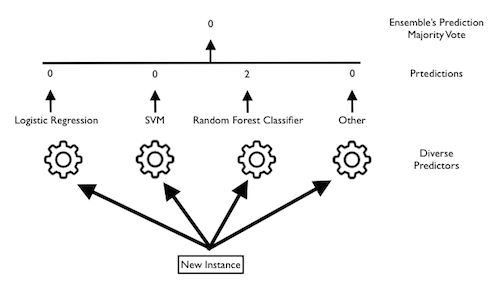
\includegraphics[width=0.9\textwidth]{images/image2.png}
            \end{figure}
        \end{column}
        \begin{column}{0.5\textwidth}
            \begin{figure}
                \centering
                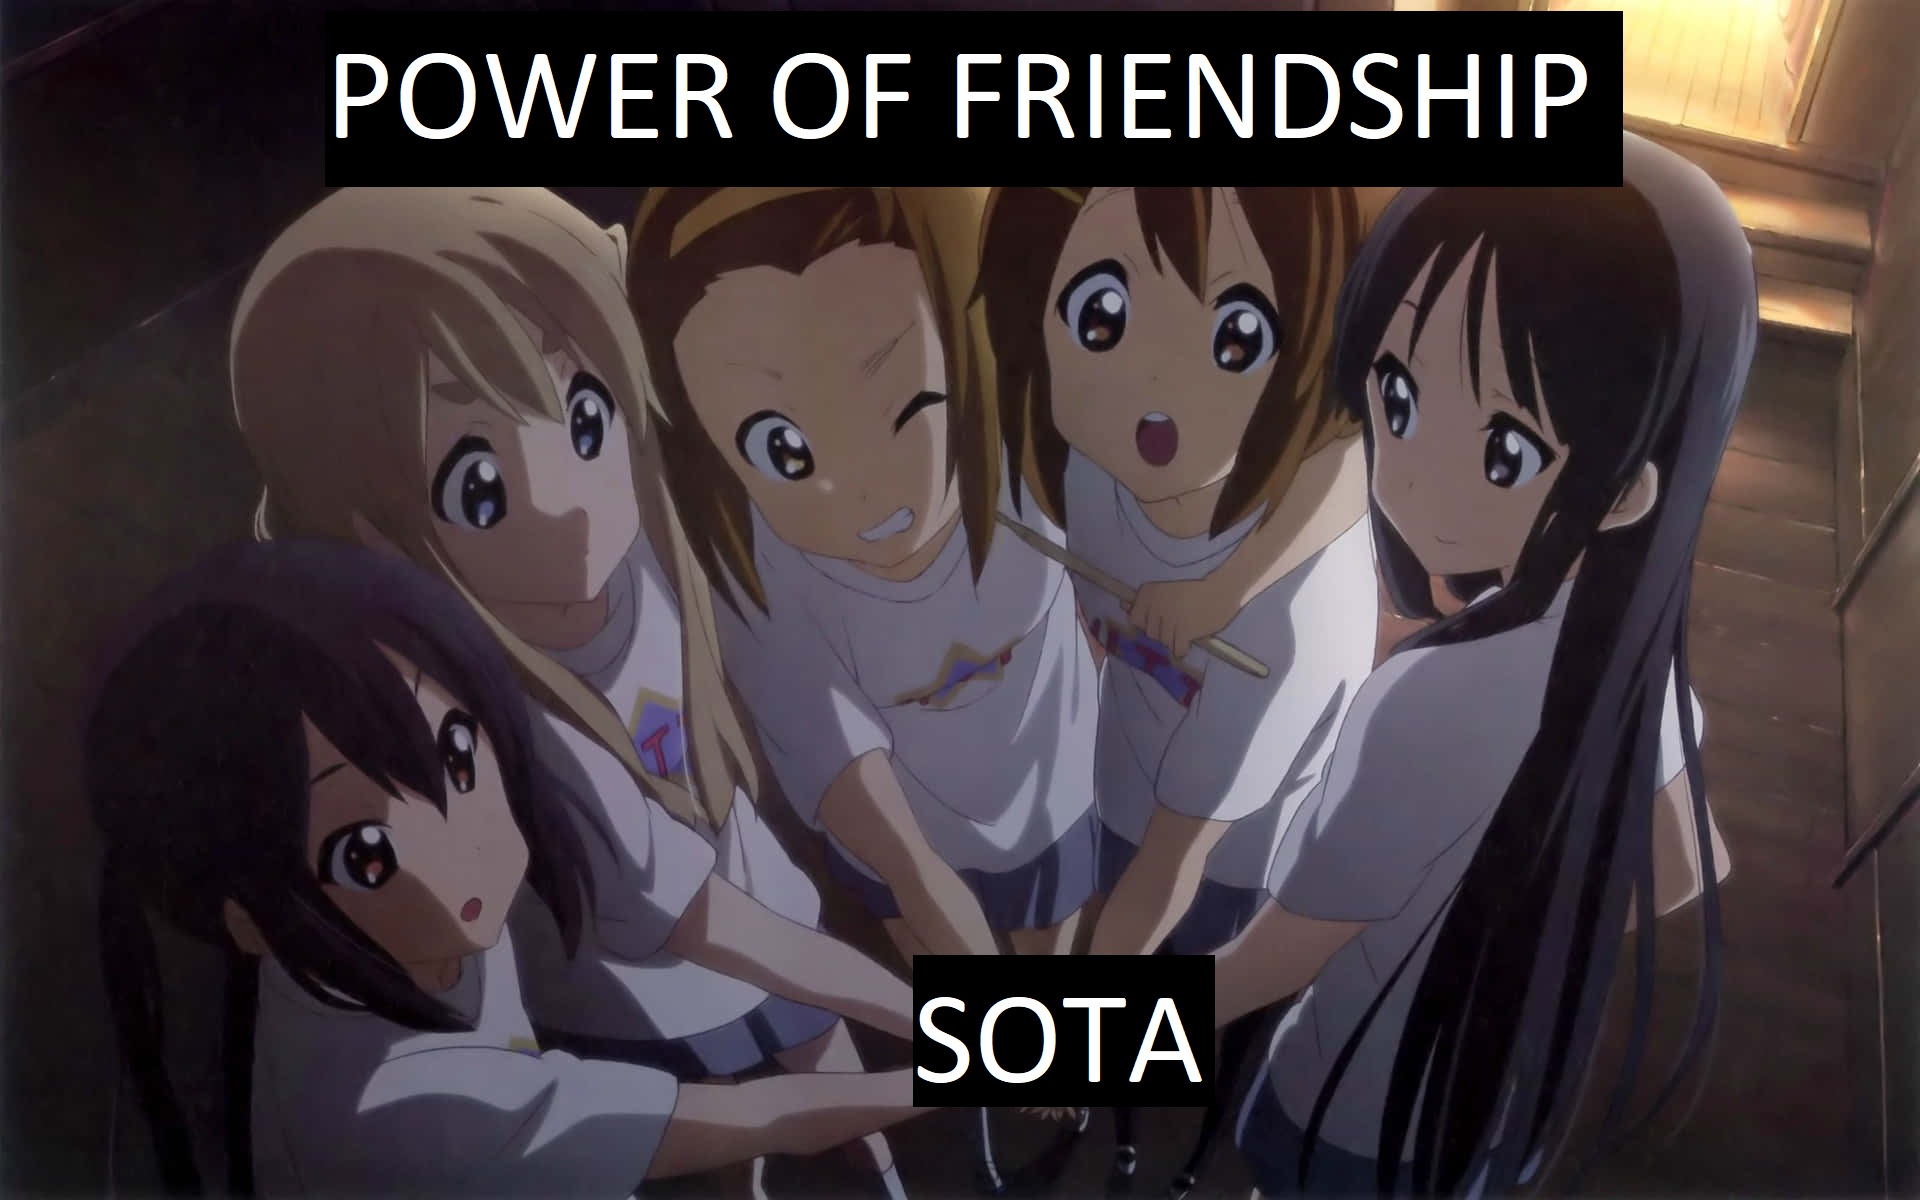
\includegraphics[width=0.9\textwidth]{images/image1.jpg}
            \end{figure}
        \end{column}
    \end{columns}
\end{frame}

\begin{frame}

    \begin{block}{ВНИМАНИЕ}
        Главный вопрос: почему ансамблирование улучшает результаты?
    \end{block}

    \begin{figure}
        \centering
        
\includegraphics[width=0.9\textwidth]{images/image3.jpg}
    \end{figure}
\end{frame}

\begin{frame}{История ансамблирования}
    \begin{block}{Подходы ансамблирования}
        \begin{enumerate}
            \item Bootstrap Aggregating (Bagging)~\cite{breiman96} --- порождает множество предикторов на случайных подвыборках данных и усредняет (или берет голос большинства) предсказания.
            \item Boosting~\cite{FREUND1997119} --- AdaBoost добавляет легкие модели по одной для компенсирования слабостей предыдущих моделей.
            \item Random Forests~\cite{random_forests} --- классика.
            \item Gradient Boosting Machine~\cite{gbm} --- классика.
            \item Stacking~\cite{WOLPERT1992241} --- мета-модель обучается на выходах базовых моделей.
        \end{enumerate}
    \end{block}
\end{frame}

\begin{frame}{В поисках ответов}
    \begin{block}{}
        Исследуем возможные объяснения эффективности ансамблей.
    \end{block}

    \begin{figure}
        \centering
        
\includegraphics[width=0.9\textwidth]{images/image4.png}
    \end{figure}
\end{frame}

\begin{frame}{Bias-Variance Decomposition}
    \begin{block}{Пусть}
        $D = \{ (x_1, y_1), \ldots, (x_n, y_n) \}, y = f(x) + \varepsilon$ и $\hat{f}(x; D)$ --- наша модель.
    \end{block}

    \begin{block}{Тогда}
        \begin{equation*}
            \mathbb{E}_{D, \varepsilon} \left[ (y - \hat{f}(x; D))^2 \right] = \left( \text{Bias}_D \left[ \hat{f}(x; D) \right] \right)^2 + \text{Var}_D \left[ \hat{f}(x; D) \right] + \sigma^2
        \end{equation*}
        где
        \begin{align*}
            &\text{Bias}_D \left[ \hat{f}(x; D) \right] = \mathbb{E}_D \left[ \hat{f}(x; D) - f(x) \right] = \mathbb{E}_D \left[ \hat{f}(x; D) \right] - \mathbb{E}_{y | x} \left[ y(x) \right] \\
            &\text{Var}_D \left[ \hat{f}(x; D) \right] = \mathbb{E}_D \left[ \left( \mathbb{E}_D \left[ \hat{f}(x; D) \right] - \hat{f}(x; D) \right)^2 \right] \\
            &\sigma^2 = \mathbb{E}_y \left[ (y - f(x))^2 \right]
        \end{align*}
    \end{block}

    \begin{block}{}
        Ансамблирование (беггинг) уменьшает Var без увеличения Bias.
    \end{block}
\end{frame}

\begin{frame}{The Condorcet Jury Theorem}
    \begin{block}{Формулировка}
        Пусть есть независимые голосующие, у каждого из которых одна и та же вероятность правильно проголосовать строго больше $1/2$. Тогда вероятность решения большинства за правильный выбор будет увеличиваться с увеличением количества голосующих (и стремиться к $1$ в пределе).
    \end{block}

    \begin{figure}
        \centering
        
\includegraphics[width=0.7\textwidth]{images/image5.jpg}
    \end{figure}
\end{frame}

\begin{frame}{Neural Tangent Kernel}
    \begin{block}{Определение}
        $f: \mathbb{R}^{D + d} \to \mathbb{R}$ --- нейронная сеть со входами $x \in \mathbb{R}^d$ и весами $W \in \mathbb{R}^D$. Тогда $f$ можно иногда аппроксимировать как \[ f(W, x) \approx f(W_0, x) + \langle W - W_0, \nabla_W f(W_0, x) \rangle \] где $W_0$ --- случайная инициализация и $\Phi_{W_0}(x) := \nabla_W f(W_0, x)$ --- neural tangent kernel.
    \end{block}

    \begin{block}<2->{Результат}
        Обучение нейронной сети $f$ аппроксимируется обучением линейной функции $\Phi_{W_0}(x)$ (kernel trick).
    \end{block}

    \begin{block}<3->{Зачем?}
        Эта двойственность позволяет использовать простые уравнения в замкнутой форме, описывающие динамику обучения, обобщение и предсказания толстых нейронных сетей.
    \end{block}
\end{frame}

\begin{frame}{NTK in Ensembles}
    
\end{frame}

\section{Дистилляция}

\begin{frame}{Knowledge Distillation}
    % https://neptune.ai/blog/knowledge-distillation
    \begin{block}{}
        \begin{itemize}
            \item Response-based knowledge
            \item Feature-based knowledge
            \item Relation-based knowledge
        \end{itemize}
    \end{block}

    \begin{figure}
        \centering
        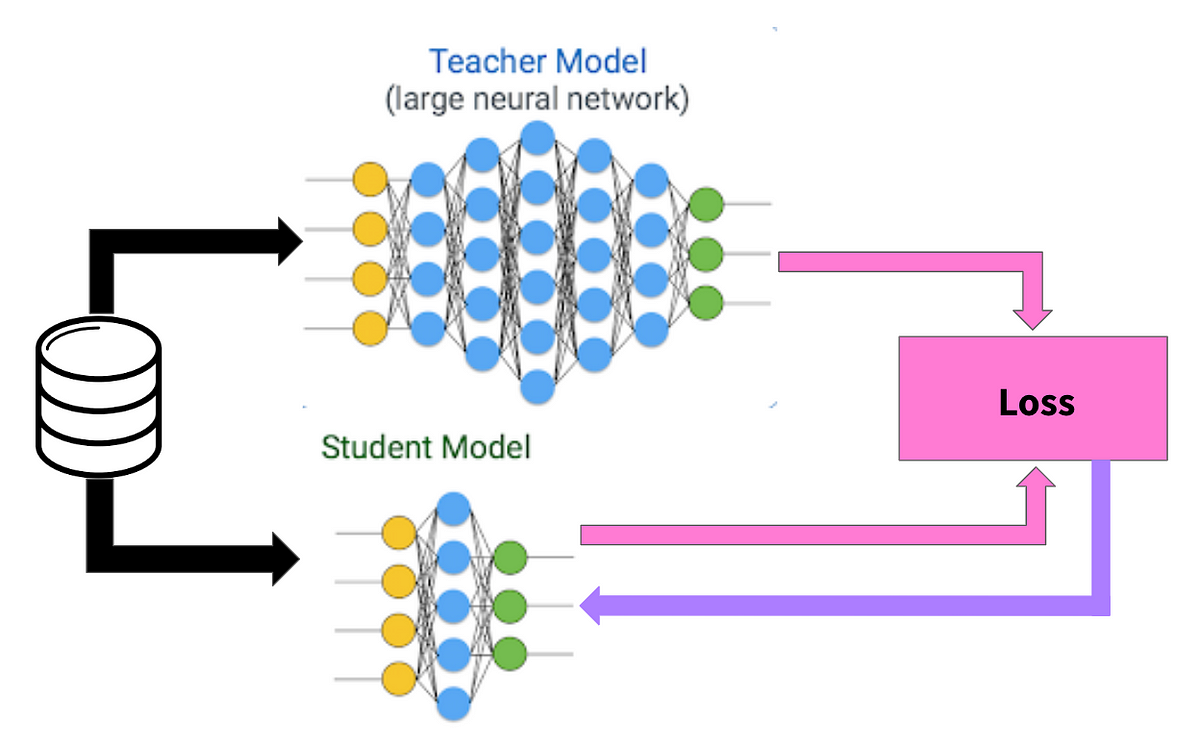
\includegraphics[width=0.7\textwidth]{images/image6.png}
    \end{figure}
\end{frame}

\begin{frame}{Практическая эффективность дистилляции~\cite{sanh2020distilbert}}

    \begin{columns}
        \begin{column}{0.5\textwidth}
            \begin{figure}
                \centering
                
\includegraphics[width=0.8\textwidth]{images/image10.png}
                \caption{Обычное обучение}
            \end{figure}
        \end{column}

        \begin{column}{0.5\textwidth}
            \begin{figure}
                \centering
                \includegraphics<2->[width=0.8\textwidth]{images/image11.png}
                \caption{Дистилляция}
            \end{figure}
        \end{column}
    \end{columns}

    \begin{figure}
        \centering
        \includegraphics<3->[width=0.7\textwidth]{images/image7.jpg}
    \end{figure}
\end{frame}

\begin{frame}{Дистилляция ансамбля~\cite{hinton2015distilling}}
    \begin{figure}
        \centering
        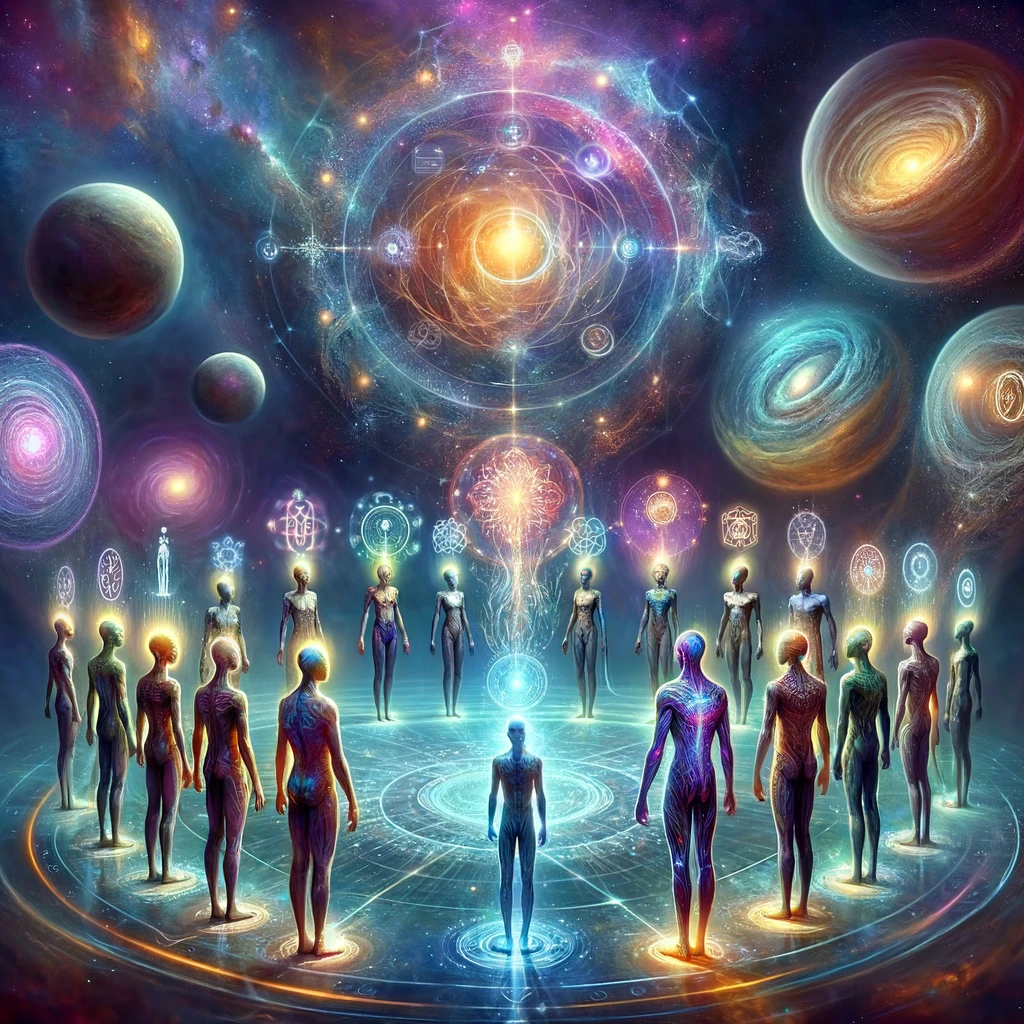
\includegraphics[width=0.5\textwidth]{images/image8.png}
    \end{figure}

    \begin{figure}
        \centering
        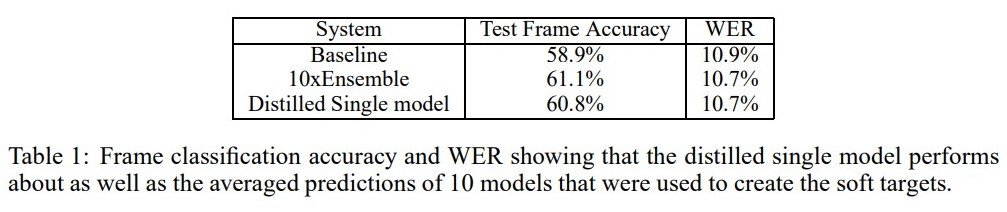
\includegraphics[width=0.8\textwidth]{images/image9.jpg}
    \end{figure}
\end{frame}

% \begin{frame}{Transfer Learning}

%     \begin{definition}
%         Применение опыта, полученного при решении одной задачи для решения новой задачи из той же области.
%     \end{definition}

%     \begin{example}<2->[Классификация изображений]
%         ResNet, обученный на ImageNet будет содержать в себе информацию о паттернах в картинках в целом, поэтому можно эту абстрактную информацию переиспользовать для решения других, более узких задач.
%     \end{example}

%     \begin{example}<3->[Языковая модель]
%         Эмбеддинги, обученные на колоссальных датасетах будут содержать в себе сложную информацию о структуре языка, поэтому их переиспользование для других задач NLP будет весьма удобным.
%     \end{example}

% \end{frame}

% \begin{frame}{Prefix-Tuning}

%     \begin{block}{Prefix-tuning}
%         Вторая рассматриваемая техника PEFT это Prefix Tuning~\cite{prefix}. Эта техника пытается решить те же проблемы, что и adapter tuning, а именно обучаться на новые задачи не теряя способности решать старые, а также обучение минимального количества весов модели\footnote{оказывается у этого есть название --- lightweight fine-tunning}, чтобы для новых задач не требовалось хранить полные копии исходной модели.
%     \end{block}

%     \begin{block}{Задачи}
%         Авторы статьи предлагают применить эту технику для задач типа table-to-text и summarization.

%         \begin{itemize}
%             \item Table-to-text --- генерация текстового описания объекта по структурированному табличному описанию. Например, из табличного представления $(\text{name}: \text{'Starbucks'}, \text{type}: \text{'coffee shop'})$ хотим получить текстовое описание: 'Starbucks serves coffee'.
%             \item Summarization --- генерация краткого текстового описания более длинного исходного текста.
%         \end{itemize}

%     \end{block}

% \end{frame}



\begin{frame}[allowframebreaks]
    \frametitle{Список литературы}
    \printbibliography
\end{frame}


\end{document}